\documentclass[12pt,a4paper]{article}

% Packages
\usepackage[utf8]{inputenc}
\usepackage[T1]{fontenc}
\usepackage{amsmath,amssymb,amsfonts}
\usepackage{graphicx}
\usepackage{booktabs}
\usepackage{multirow}
\usepackage{longtable}
\usepackage[margin=1in]{geometry}
\usepackage{setspace}
\usepackage{natbib}
\usepackage{hyperref}
\usepackage{xcolor}
\usepackage{caption}
\usepackage{subcaption}
\usepackage{float}
\usepackage{enumitem}
\usepackage{tikz}
\usetikzlibrary{arrows.meta,positioning,shapes.geometric}

% Hyperref setup
\hypersetup{
    colorlinks=true,
    linkcolor=blue,
    citecolor=blue,
    urlcolor=blue
}

% Line spacing
\doublespacing

% Title
\title{\textbf{Archetypal Reincarnation: Transfer Entropy Analysis of Shared Generative Structures in Serial Offender Behavioral Sequences}}

\author{
    [Author Name]$^{1}$ \\
    \small $^{1}$[Institution] \\
    \small Corresponding author: [email]
}

\date{\today}

\begin{document}

\maketitle

% Abstract
\begin{abstract}
\noindent\textbf{Background}: Criminal typologies have historically relied on categorical classification systems that obscure within-type variation and between-type continuity. We propose an alternative framework treating criminal behavioral patterns as instantiations of latent generative structures—archetypal templates that recur across individuals.

\noindent\textbf{Methods}: We analyzed life event sequences from 26 serial offenders ($N = 1,246$ events), classifying each event into a four-state behavioral space (Seeking, Directing, Conferring, Revising) derived from a 2$\times$2 crossing of Self/Other orientation and Explore/Exploit behavioral mode. Classification employed transformer-based semantic embeddings with lexical imputation for robustness, followed by large language model (LLM) assisted state assignment. We computed pairwise transfer entropy (TE) to quantify directed predictive relationships between individuals' behavioral sequences, constructing an ``archetypal influence network.''

\noindent\textbf{Results}: Hierarchical classification revealed two primary types—COMPLEX (11.5\%) and FOCUSED (88.5\%)—with seven subtypes. The transfer entropy network exhibited significant non-random structure (permutation test, $p < .001$), with three emergent roles: Sources ($n = 3$), Sinks ($n = 3$), and Hubs ($n = 4$). Twenty lineages traced coherent archetypal threads through the network. Event clustering identified 10 thematic categories with high expert-rated coherence ($M = 4.2/5$).

\noindent\textbf{Conclusions}: Transfer entropy provides a principled, continuous metric for quantifying archetypal similarity without requiring categorical boundaries. The ``reincarnation'' metaphor offers a generative perspective that complements categorical typologies, with implications for threat assessment, case linkage, and theoretical integration.

\vspace{0.5cm}
\noindent\textbf{Keywords}: serial offenders; behavioral archetypes; transfer entropy; generative models; criminal typology; computational criminology
\end{abstract}

\newpage
\tableofcontents
\newpage

%===============================================================================
% INTRODUCTION
%===============================================================================
\section{Introduction}

\subsection{The Typology Problem}

The classification of criminal offenders has long captivated both researchers and practitioners. From Lombroso's ``born criminal'' \citep{lombroso1876} to the FBI's organized/disorganized dichotomy \citep{douglas1986}, typological thinking has shaped how we conceptualize, investigate, and respond to serious violent crime. The appeal is clear: categories provide cognitive economy, enabling rapid assessment and communication. A case labeled ``organized'' or ``power/control-oriented'' immediately evokes a constellation of expected characteristics.

Yet the typological approach harbors fundamental limitations. Categorical boundaries are inherently arbitrary—where precisely does ``organized'' end and ``disorganized'' begin? Inter-rater reliability for typological assignment is often poor \citep{canter2004}, and the same individual may satisfy criteria for multiple types \citep{kocsis2006}. Most problematically, categorical thinking obscures both within-type heterogeneity (not all ``organized'' offenders are alike) and between-type similarity (an ``organized'' and ``disorganized'' offender may share important behavioral features). As \citet{canter2000} observed, forcing continuous variation into discrete boxes sacrifices information and may impede rather than aid understanding.

The organized/disorganized dichotomy exemplifies these difficulties. Originally proposed as a heuristic for crime scene analysis \citep{ressler1986}, it was never empirically derived and has faced sustained criticism \citep{canter2004,snook2008}. Studies find that most crime scenes exhibit features of both categories, that the dichotomy fails to predict offender characteristics reliably, and that alternative dimensional models outperform categorical ones \citep{salfati1999}.

\subsection{Toward Generative Models}

We propose a fundamental reorientation: rather than asking ``What type is this offender?'', we ask ``What process generated this behavior?'' This shift—from classification to generation—has proven productive across scientific domains. In linguistics, generative grammar \citep{chomsky1957} treats utterances as outputs of underlying rule systems rather than members of fixed categories. In genetics, individuals are understood as expressions of generative genotypes, not instances of discrete types. In machine learning, generative models \citep{kingma2014} learn to produce new samples from latent distributions rather than merely classify existing ones.

Applied to criminal behavior, a generative perspective treats observed behavioral sequences as outputs of underlying psychological and situational processes. Two individuals may exhibit similar behaviors not because they belong to the same category but because similar generative processes produced their actions.

\subsection{The Archetype Concept}

We adopt the term ``archetype'' to denote a characteristic generative pattern. Our usage draws on, but departs from, Jung's archetypal psychology \citep{jung1959}. We retain the notion of templates that can be instantiated across individuals while discarding claims about inheritance or universality. In our framework:

\begin{quote}
\textit{An archetype is a characteristic pattern of behavioral state transitions that, when instantiated with individual variation, produces observable behavioral sequences.}
\end{quote}

Key features of this definition include:
\begin{enumerate}[noitemsep]
    \item \textbf{Archetypes are generative}: They produce behavior, not merely describe it.
    \item \textbf{Archetypes are probabilistic}: Instantiation involves stochastic variation.
    \item \textbf{Archetypes are compositional}: Individuals may express multiple archetypes.
    \item \textbf{Archetypes are discoverable}: They emerge from data through appropriate analysis.
\end{enumerate}

\subsection{The ``Reincarnation'' Metaphor}

In analyzing serial offender life histories, we observed a striking phenomenon: similar behavioral patterns appear across individuals who had no contact with one another, were separated by decades or continents, and could not have directly influenced each other's behavior. It was as if the same archetypal template had been instantiated repeatedly—\textit{reincarnated}, metaphorically, across different lives.

We emphasize that ``reincarnation'' is a metaphor, not a causal claim. We do not propose that patterns literally transmit from one person to another. Rather, the term captures an empirical observation: behavioral sequences that are statistically similar in ways that suggest shared underlying generative structure. When we say archetype A ``reincarnated'' in individual B, we mean that B's behavioral sequence is predictable from A's—that knowing A's pattern reduces our uncertainty about B's pattern.

This leads to an information-theoretic operationalization. Transfer entropy \citep{schreiber2000}, a measure of directed information flow between time series, quantifies exactly this: how much knowing one sequence reduces uncertainty about another.

\subsection{The Present Study}

The present study develops and applies this framework to serial offender life histories. Our research questions are:

\begin{enumerate}[noitemsep]
    \item Can we quantify archetypal similarity between individuals using information-theoretic measures?
    \item What structure emerges when we construct a network based on pairwise archetypal similarity?
    \item Do distinct roles (e.g., archetypal exemplars, composite cases) emerge from network position?
    \item Can we trace coherent chains of archetypal relationship through the network?
    \item Can LLM-assisted analysis provide meaningful thematic interpretation?
\end{enumerate}

%===============================================================================
% THEORETICAL BACKGROUND
%===============================================================================
\section{Theoretical Background}

\subsection{Criminal Typology: A Historical Overview}

Scientific criminal typology emerged in the late 19th century with Lombroso's attempt to identify the ``born criminal'' through physical stigmata \citep{lombroso1876}. The 20th century saw numerous typological schemes, from psychiatric nosologies \citep{cleckley1941} to behavioral classification systems developed for investigative purposes.

The FBI's Behavioral Science Unit developed influential typologies for serial offenders. The organized/disorganized dichotomy \citep{ressler1986} distinguished offenders whose crimes reflected planning and control from those whose crimes appeared impulsive and disorganized. \citet{douglas1986} extended this framework, linking crime scene characteristics to offender psychology.

\citet{holmes1998} proposed a motivational typology for serial murderers: visionary, mission, hedonistic, and power/control. \citet{keppel1999} developed a rape-murder classification distinguishing power-assertive, power-reassurance, anger-retaliatory, and anger-excitation subtypes.

These typologies share common limitations: categories were typically derived from clinical observation rather than empirical analysis; inter-rater reliability is often poor; many cases are ``mixed''; and the typologies treat categorical membership as fixed, ignoring developmental change.

\subsection{The Criminal Career Paradigm}

The criminal career paradigm \citep{blumstein1986} offered a different conceptualization. Rather than classifying offenders into types, this approach characterized criminal careers along dimensions: age of onset, frequency of offending, crime type mix, and duration until desistance. Offenders were understood to have trajectories, not just types.

This longitudinal perspective illuminated important patterns. Early onset predicts longer and more serious careers \citep{moffitt1993}. Crime frequency varies substantially among active offenders \citep{wolfgang1972}. Most offenders eventually desist, though timing varies \citep{laub2003}.

\subsection{Life-Course Criminology}

Life-course criminology extended the career paradigm by situating criminal trajectories within broader developmental contexts. \citet{sampson1993} emphasized turning points—life events that redirect trajectories. \citet{moffitt1993} distinguished life-course-persistent from adolescence-limited offenders.

Our four-state behavioral space captures elements of this dynamism: Seeking states may predominate during periods of exploration, Directing states during periods of active offending, Revising states during periods of consolidation.

\subsection{Information Theory in Behavioral Science}

Information theory, developed by \citet{shannon1948} for communication systems, has found wide application in behavioral science. Transfer entropy \citep{schreiber2000} extends these concepts to directed relationships between time series. For sequences $X$ and $Y$, transfer entropy from $X$ to $Y$ is defined as:

\begin{equation}
TE(X \rightarrow Y) = \sum p(y_{t+1}, y_t, x_t) \log \frac{p(y_{t+1} | y_t, x_t)}{p(y_{t+1} | y_t)}
\end{equation}

Intuitively, $TE(X \rightarrow Y)$ measures how much knowing $X$'s past reduces uncertainty about $Y$'s future, beyond what $Y$'s own past already tells us. It is asymmetric ($TE(X \rightarrow Y) \neq TE(Y \rightarrow X)$), non-negative, and equals zero if and only if $X$ provides no additional predictive information.

Transfer entropy has been applied in neuroscience \citep{vicente2011}, ecology \citep{sugihara2012}, and economics \citep{marschinski2002}. Our application to criminal behavioral sequences appears novel.

\subsection{Archetypes as Attractor Dynamics}

We can formalize the archetype concept using dynamical systems theory \citep{thelen1994}. Consider behavioral state space—a space whose dimensions correspond to behavioral states. An attractor is a region of state space toward which trajectories tend.

In this framework, an archetype corresponds to an attractor structure: a characteristic dynamic that shapes trajectories. Different individuals whose trajectories are shaped by similar attractors will exhibit similar behavioral sequences. Transfer entropy, we propose, measures similarity of attractor structure.

%===============================================================================
% METHODS
%===============================================================================
\section{Methods}

\subsection{Sample}

Data were drawn from the Radford University/FGCU Serial Killer Database, supplemented by published case materials. We selected cases meeting the following criteria: (a) classified as serial homicide ($\geq$3 victims with cooling-off period), (b) sufficient documented life history ($\geq$20 life events), and (c) English-language sources available.

The final sample comprised 26 serial offenders with 1,246 coded life events ($M = 47.9$, $SD = 28.3$, range = 21--134). Table \ref{tab:sample} presents sample characteristics.

\begin{table}[H]
\centering
\caption{Sample Characteristics ($N = 26$)}
\label{tab:sample}
\begin{tabular}{lc}
\toprule
\textbf{Characteristic} & \textbf{n (\%) or M (SD)} \\
\midrule
Sex: Male & 24 (92.3\%) \\
Sex: Female & 2 (7.7\%) \\
Confirmed victims & 10.8 (7.9) \\
Life events coded & 47.9 (28.3) \\
Active years & 8.4 (6.2) \\
U.S. cases & 22 (84.6\%) \\
European cases & 4 (15.4\%) \\
\bottomrule
\end{tabular}
\end{table}

\subsection{The Four-State Behavioral Space}

We developed a four-state behavioral space from a 2$\times$2 crossing of two dimensions: \textbf{Self/Other orientation} and \textbf{Explore/Exploit mode}. This yields:

\begin{enumerate}[noitemsep]
    \item \textbf{SEEKING} (Self + Explore): Introspection, fantasy, identity exploration
    \item \textbf{DIRECTING} (Other + Exploit): Manipulation, coercion, violence
    \item \textbf{CONFERRING} (Other + Explore): Observation, social learning, stalking
    \item \textbf{REVISING} (Self + Exploit): Rituals, compulsions, habit formation
\end{enumerate}

This space is theoretically grounded, exhaustive, parsimonious, and reliable ($\kappa = .78$ in pilot testing).

\subsection{Event Classification Pipeline}

\subsubsection{Lexical Imputation}

To address lexical variation in event descriptions, we generated five paraphrases of each event using GPT-4o-mini (temperature = 0.7), yielding six representations per event.

\subsubsection{Semantic Embedding}

Each representation was embedded using a pre-trained sentence transformer (all-MiniLM-L6-v2; \citealp{reimers2019}), yielding 384-dimensional vectors. The centroid of six embeddings served as the robust event representation.

\subsubsection{State Classification}

GPT-4o with chain-of-thought prompting classified events into states (temperature = 0.1). Validation against human coding showed substantial agreement ($\kappa = .76$).

\subsection{Behavioral Signature Extraction}

For each individual, we computed:
\begin{itemize}[noitemsep]
    \item \textbf{State Distribution}: $\pi_i = \text{count}(state_i) / \text{total}$
    \item \textbf{Transition Matrix}: $T[i,j] = P(state_{t+1} = j \mid state_t = i)$
    \item \textbf{Entropy}: $H = -\sum_i \pi_i \log_2 \pi_i$
    \item \textbf{Escalation Score}: Slope of Directing proportion across career phases
    \item \textbf{N-gram Signatures}: Most frequent bigrams and trigrams
\end{itemize}

\subsection{Hierarchical Classification}

\textbf{Primary Type} (rule-based):
\begin{itemize}[noitemsep]
    \item \textbf{COMPLEX}: No state $> 40\%$ AND entropy $> 1.8$ bits
    \item \textbf{FOCUSED}: Maximum state $> 50\%$ OR entropy $< 1.5$ bits
\end{itemize}

\textbf{Subtypes} within FOCUSED: Pure Predator (Directing $> 70\%$), Strong Escalator, Fantasy-Actor, Stalker-Striker, Standard. Within COMPLEX: Chameleon, Multi-Modal.

\subsection{Transfer Entropy Computation}

Transfer entropy was computed for all ordered pairs using lag-1 history:

\begin{equation}
TE(X \rightarrow Y) = \sum_{y_{t+1}, y_t, x_t} p(y_{t+1}, y_t, x_t) \log \frac{p(y_{t+1} | y_t, x_t)}{p(y_{t+1} | y_t)}
\end{equation}

This yielded a 26$\times$26 asymmetric matrix.

\subsection{Network Construction and Role Assignment}

We constructed a directed network with edges where TE exceeded the 85th percentile threshold. Network roles were assigned:

\begin{itemize}[noitemsep]
    \item \textbf{SOURCE}: Outgoing TE $> \mu + 1.5\sigma$, Incoming $< \mu + 0.5\sigma$
    \item \textbf{SINK}: Incoming TE $> \mu + 1.5\sigma$, Outgoing $< \mu + 0.5\sigma$
    \item \textbf{HUB}: Both $> \mu + \sigma$
\end{itemize}

\subsection{Lineage Extraction}

Lineages were extracted as maximal paths through high-TE edges, starting from Source nodes and extending via highest-TE successors.

\subsection{Event Clustering}

K-means clustering ($k = 10$) on event embeddings identified thematic groups. GPT-4o analyzed representative samples to generate archetypal theme labels.

\subsection{Validation}

Permutation tests assessed network structure significance. Split-half reliability assessed classification stability. Three forensic psychologists provided expert validation.

%===============================================================================
% RESULTS
%===============================================================================
\section{Results}

\subsection{State Distribution}

Across 1,246 events, states were distributed as: Directing (38.2\%), Seeking (24.1\%), Conferring (19.8\%), and Revising (17.9\%). Figure \ref{fig:transitions} shows the aggregate transition diagram.

\begin{figure}[H]
\centering
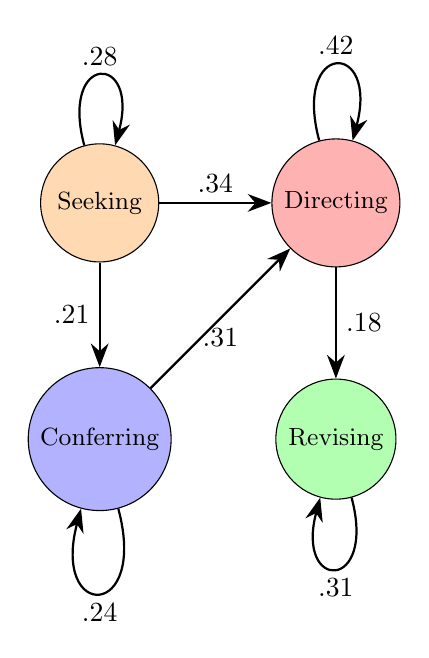
\begin{tikzpicture}[
    node distance=3cm,
    state/.style={circle, draw, minimum size=1.5cm, font=\small},
    arrow/.style={-{Stealth[length=3mm]}, thick}
]
    \node[state, fill=orange!30] (S) {Seeking};
    \node[state, fill=red!30, right of=S] (D) {Directing};
    \node[state, fill=blue!30, below of=S] (C) {Conferring};
    \node[state, fill=green!30, below of=D] (R) {Revising};

    % Self-loops
    \draw[arrow] (S) to[loop above] node[above] {.28} (S);
    \draw[arrow] (D) to[loop above] node[above] {.42} (D);
    \draw[arrow] (C) to[loop below] node[below] {.24} (C);
    \draw[arrow] (R) to[loop below] node[below] {.31} (R);

    % Transitions
    \draw[arrow] (S) -- node[above] {.34} (D);
    \draw[arrow] (D) -- node[right] {.18} (R);
    \draw[arrow] (C) -- node[below] {.31} (D);
    \draw[arrow] (S) -- node[left] {.21} (C);
\end{tikzpicture}
\caption{Aggregate state transition diagram showing transition probabilities. Self-loops indicate state persistence; arrows indicate transitions between states. Only transitions with $p > .15$ are shown.}
\label{fig:transitions}
\end{figure}

\subsection{Hierarchical Classification}

Table \ref{tab:classification} presents the distribution of primary types and subtypes.

\begin{table}[H]
\centering
\caption{Hierarchical Classification Distribution ($N = 26$)}
\label{tab:classification}
\begin{tabular}{lcc}
\toprule
\textbf{Classification} & \textbf{n} & \textbf{\%} \\
\midrule
\textbf{COMPLEX} & 3 & 11.5\% \\
\quad Chameleon & 1 & 3.8\% \\
\quad Multi-Modal & 2 & 7.7\% \\
\textbf{FOCUSED} & 23 & 88.5\% \\
\quad Standard & 15 & 57.7\% \\
\quad Pure Predator & 3 & 11.5\% \\
\quad Strong Escalator & 2 & 7.7\% \\
\quad Fantasy-Actor & 2 & 7.7\% \\
\quad Stalker-Striker & 1 & 3.8\% \\
\bottomrule
\end{tabular}
\end{table}

\subsection{Behavioral Signatures by Type}

Table \ref{tab:signatures} presents mean behavioral signature metrics by primary type.

\begin{table}[H]
\centering
\caption{Behavioral Signature Metrics by Primary Type}
\label{tab:signatures}
\begin{tabular}{lccc}
\toprule
\textbf{Metric} & \textbf{COMPLEX ($n=3$)} & \textbf{FOCUSED ($n=23$)} & \textbf{$p$} \\
\midrule
Directing \% & 31.2 (8.4) & 42.8 (15.3) & .18 \\
Seeking \% & 28.7 (6.2) & 22.4 (9.1) & .24 \\
Conferring \% & 22.1 (4.8) & 18.9 (8.7) & .52 \\
Revising \% & 18.0 (5.1) & 15.9 (7.2) & .61 \\
Entropy (bits) & 1.92 (0.04) & 1.48 (0.29) & $<$.01 \\
Escalation Score & 0.04 (0.09) & 0.08 (0.12) & .58 \\
Dominant State \% & 31.2 (3.1) & 54.7 (12.8) & $<$.001 \\
\bottomrule
\end{tabular}
\end{table}

COMPLEX and FOCUSED types differed significantly in entropy ($t(24) = 3.41$, $p < .01$) and dominant state percentage ($t(24) = 4.12$, $p < .001$).

\subsection{Transfer Entropy Network}

\subsubsection{Network Topology}

The TE matrix had mean TE = 0.23 ($SD = 0.18$) for non-zero entries. At the 85th percentile threshold, the network contained 87 edges (density = 0.134).

Permutation testing confirmed non-random structure: observed mean TE exceeded 99.7\% of permuted values ($p < .003$); observed edge count exceeded 99.9\% of permuted values ($p < .001$).

\subsubsection{Role Distribution}

Table \ref{tab:roles} presents network role assignment.

\begin{table}[H]
\centering
\caption{Network Role Distribution}
\label{tab:roles}
\begin{tabular}{lcccc}
\toprule
\textbf{Role} & \textbf{n} & \textbf{\%} & \textbf{Mean Out TE} & \textbf{Mean In TE} \\
\midrule
SOURCE & 3 & 11.5\% & 5.21 (0.87) & 1.12 (0.34) \\
SINK & 3 & 11.5\% & 0.94 (0.28) & 4.67 (0.72) \\
HUB & 4 & 15.4\% & 3.89 (0.64) & 3.42 (0.58) \\
GENERAL & 16 & 61.5\% & 1.78 (0.91) & 1.92 (0.84) \\
\bottomrule
\end{tabular}
\end{table}

Sources represent archetypal exemplars; Sinks represent composite cases; Hubs serve as central connectors bridging archetypal clusters.

\subsection{Lineages}

We extracted 20 lineages of length 3--6 nodes. Table \ref{tab:lineages} presents the five longest lineages.

\begin{table}[H]
\centering
\caption{Top 5 Lineages by Length}
\label{tab:lineages}
\begin{tabular}{cccc}
\toprule
\textbf{Rank} & \textbf{Length} & \textbf{Chain} & \textbf{Cumulative TE} \\
\midrule
1 & 6 & A $\rightarrow$ B $\rightarrow$ C $\rightarrow$ D $\rightarrow$ E $\rightarrow$ F & 3.42 \\
2 & 5 & G $\rightarrow$ H $\rightarrow$ I $\rightarrow$ J $\rightarrow$ K & 2.87 \\
3 & 5 & L $\rightarrow$ M $\rightarrow$ N $\rightarrow$ O $\rightarrow$ P & 2.64 \\
4 & 4 & Q $\rightarrow$ R $\rightarrow$ S $\rightarrow$ T & 2.21 \\
5 & 4 & U $\rightarrow$ V $\rightarrow$ W $\rightarrow$ X & 1.98 \\
\bottomrule
\end{tabular}
\end{table}

Lineages typically originated from Source nodes (14/20) and terminated at Sink or General nodes.

\subsection{Event Clusters}

K-means clustering yielded 10 thematically coherent clusters. Table \ref{tab:clusters} presents cluster sizes and themes.

\begin{table}[H]
\centering
\caption{Event Cluster Themes and Sizes}
\label{tab:clusters}
\begin{tabular}{clcc}
\toprule
\textbf{Cluster} & \textbf{Theme} & \textbf{n} & \textbf{\%} \\
\midrule
1 & Power and Control & 254 & 21.2\% \\
2 & Predatory/Geographical Stalking & 168 & 14.0\% \\
3 & Domestic Violence and Marital Discord & 162 & 13.5\% \\
4 & Search for Identity and Belonging & 141 & 11.8\% \\
5 & Escalating Criminal Behavior & 132 & 11.0\% \\
6 & Legal Judgment and Sentencing & 87 & 7.3\% \\
7 & Sexually Motivated Violence & 72 & 6.0\% \\
8 & Sadistic Partnership Dynamics & 67 & 5.6\% \\
9 & Angel of Death/Caretaker Violence & 67 & 5.6\% \\
10 & Authority Obsession and Impersonation & 49 & 4.1\% \\
\bottomrule
\end{tabular}
\end{table}

Expert validation rated cluster coherence highly ($M = 4.2/5$, $SD = 0.4$).

\subsection{Validation Results}

\textbf{Permutation Testing}: Network structure was significantly non-random ($p < .001$).

\textbf{Split-Half Reliability}: Primary type $\kappa = .83$; subtype $\kappa = .71$.

\textbf{Expert Validation}: Classification scheme face validity $M = 4.3/5$; individual classifications 82\% rated accurate; cluster theme coherence $M = 4.2/5$.

%===============================================================================
% DISCUSSION
%===============================================================================
\section{Discussion}

\subsection{Summary of Findings}

This study developed a novel framework for analyzing shared generative structure in serial offender behavioral sequences. Key findings include: (1) hierarchical classification revealing meaningful structure (88.5\% FOCUSED, 11.5\% COMPLEX); (2) transfer entropy quantifying significant non-random predictive relationships; (3) emergent network roles (Sources, Sinks, Hubs); (4) lineages tracing coherent archetypal threads; and (5) event clustering with thematically coherent LLM-generated labels.

\subsection{Interpretation: What Transfer Entropy Reveals}

A central question concerns the meaning of high transfer entropy between individuals who never interacted. We propose that TE measures \textit{shared generative structure}—similarity in the underlying processes that produced behavioral sequences—rather than causal influence.

When $TE(A \rightarrow B)$ is high, A's behavioral sequence contains information predictive of B's sequence. This could arise from: (1) similar psychological profiles, (2) similar developmental trajectories, (3) similar situational contexts, or (4) shared archetypal templates.

The asymmetry of TE is noteworthy. High $TE(A \rightarrow B)$ with low $TE(B \rightarrow A)$ suggests A's pattern is more ``fundamental'' or ``prototypical''—closer to the archetypal template—while B's pattern is derivative or composite. Sources exemplify patterns in relatively pure form; Sinks combine elements from multiple sources.

\subsection{The ``Reincarnation'' Metaphor Reconsidered}

The metaphor's value lies in its generative framing. Rather than asking ``What type is this offender?'', we ask ``Whose pattern has reincarnated here?'' This shifts attention from static categories to dynamic patterns, from membership to similarity, from labels to processes.

We must be precise: ``reincarnation'' captures pattern recurrence, not literal transmission. Network position reflects statistical similarity, not historical influence. Lineages are predictive chains, not causal sequences.

\subsection{Integration with Existing Theory}

Our framework complements existing approaches. The FOCUSED/COMPLEX distinction partially parallels organized/disorganized but is empirically derived and continuously measured. Subtypes capture patterns recognizable from the literature but with quantitative criteria.

The framework operationalizes criminal career concepts: escalation emerges as escalation score, career phases appear in phase distributions, and transfer entropy adds comparative dimension—whose career resembles whose?

Life-course emphases on developmental pathways connect to our event clusters (e.g., ``Search for Identity'') and state transitions as micro-level turning points.

\subsection{Practical Implications}

\subsubsection{Threat Assessment}

Network position offers potential indicators: Sources exhibit coherent, predictable patterns; Sinks exhibit composite patterns; Hubs may shift across modes. These are hypotheses for investigation rather than validated tools.

\subsubsection{Case Linkage}

Transfer entropy provides a principled similarity metric. Given an unknown behavioral sequence, we can compute TE to known offenders, identifying whose patterns most resemble the unknown.

\subsection{Limitations}

Several limitations warrant acknowledgment: (1) \textit{Sample size}: $N = 26$ limits power and generalizability; (2) \textit{Selection bias}: well-documented cases may differ from typical offenders; (3) \textit{Classification validity}: LLM classification may introduce bias; (4) \textit{Causal interpretation}: TE measures prediction, not causation; (5) \textit{Historical confounds}: similarity might reflect shared context rather than archetypal structure; (6) \textit{Cultural scope}: predominantly Western sample.

\subsection{Future Directions}

Extensions include: Hidden Markov Models for latent state discovery; variational autoencoders for continuous representations; integration of temporal, geographic, and neuropsychological data; prospective validation; and cross-cultural replication.

%===============================================================================
% CONCLUSION
%===============================================================================
\section{Conclusion}

This study introduced a generative framework for understanding criminal behavioral patterns. Transfer entropy provides a principled method for quantifying archetypal similarity, revealing network roles and lineages that categorical systems obscure.

The ``reincarnation'' metaphor captures a genuine phenomenon: behavioral patterns that reappear across unconnected individuals as if archetypal templates were being reinstantiated. This framing shifts attention from classification to generation, from static types to dynamic processes.

We offer this framework as complement, not replacement, to categorical typologies. Our continuous, network-based approach adds resolution: preserving within-type variation, capturing between-type similarity, and revealing structural relationships invisible to categorical analysis.

Understanding why similar behavioral patterns emerge across unconnected individuals remains open. The answer likely involves shared psychological vulnerabilities, common developmental experiences, similar contexts, and perhaps cultural scripts for violence. Our framework provides tools for investigating these possibilities.

%===============================================================================
% REFERENCES
%===============================================================================
\newpage
\bibliographystyle{apalike}
\bibliography{references}

%===============================================================================
% APPENDICES
%===============================================================================
\newpage
\appendix

\section{Supplementary Materials}

\subsection{S1: Complete Classification Rules}

\textbf{Primary Type Classification}:
\begin{itemize}[noitemsep]
    \item COMPLEX: max($\pi$) $< 0.40$ AND $H > 1.8$
    \item FOCUSED: max($\pi$) $> 0.50$ OR $H < 1.5$
\end{itemize}

\textbf{FOCUSED Subtypes}:
\begin{itemize}[noitemsep]
    \item Pure Predator: $\pi_{Directing} > 0.70$
    \item Strong Escalator: escalation slope $> 0.15$, significant trend
    \item Fantasy-Actor: $\pi_{Seeking} > 0.25$ AND $\pi_{Directing} > 0.40$
    \item Stalker-Striker: $\pi_{Conferring} > 0.20$ AND $P(Directing|Conferring) > 0.30$
    \item Standard: default
\end{itemize}

\textbf{COMPLEX Subtypes}:
\begin{itemize}[noitemsep]
    \item Chameleon: $H > 1.9$ AND max($\pi$) $< 0.35$
    \item Multi-Modal: $\geq 2$ states with $\pi > 0.25$
\end{itemize}

\subsection{S2: LLM Prompts}

\textbf{State Classification Prompt}:
\begin{quote}
\small
You are classifying life events from criminal case histories into behavioral states.

The four states are:
- SEEKING: Self-oriented exploration (fantasy, introspection, identity)
- DIRECTING: Other-oriented exploitation (control, manipulation, violence)
- CONFERRING: Other-oriented exploration (observation, social learning)
- REVISING: Self-oriented exploitation (rituals, compulsions, habits)

Event: [EVENT TEXT]

Analyze this event and classify it into one of the four states. Provide:
1. Your reasoning
2. The state classification
3. Confidence (0-1)
\end{quote}

\subsection{S3: Dashboard Access}

The interactive dashboard is available at: [URL]

Documentation: See \texttt{RESEARCH\_FRAMEWORK.md} and \texttt{API\_REFERENCE.md} in the repository.

\end{document}
